\documentclass{article}
\usepackage{graphicx}
\usepackage{float}
\usepackage{subcaption}
\usepackage[utf8]{inputenc}
\usepackage[margin=1in]{geometry}

\title{Perceptron with Hebbian Learning - Report}
\author{Brum}
\date{\today}

\begin{document}

\maketitle

\section{Introduction}
This report analyzes the performance of a Perceptron trained using the Hebb rule on three different datasets. The model was evaluated based on accuracy, training error evolution, and decision boundary visualization (for 2D datasets).

\section{Dataset 1}

\subsection{Results}
\begin{itemize}
    \item \textbf{Training Accuracy (Last Epoch):} 96.43\%
    \item \textbf{Test Accuracy:} 95.00\%
\end{itemize}

\subsection{Analysis}
The model achieved high accuracy on both training and test sets. As observed in the decision boundary plots below, the data is almost linearly separable, allowing the Perceptron to find a hyperplane that correctly classifies most samples. The training error converged quickly (as seen in the error evolution graph).

\begin{figure}[H]
    \centering
    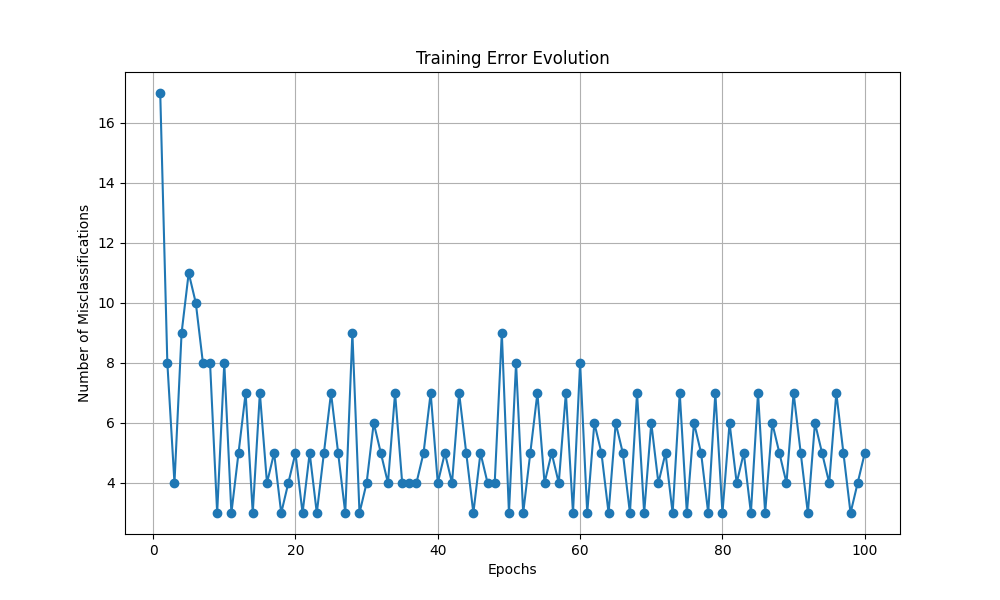
\includegraphics[width=0.7\textwidth]{output/dataset1/training_error.png}
    \caption{Dataset 1: Training Error Evolution}
\end{figure}

\begin{figure}[H]
    \centering
    \begin{subfigure}[b]{0.48\textwidth}
        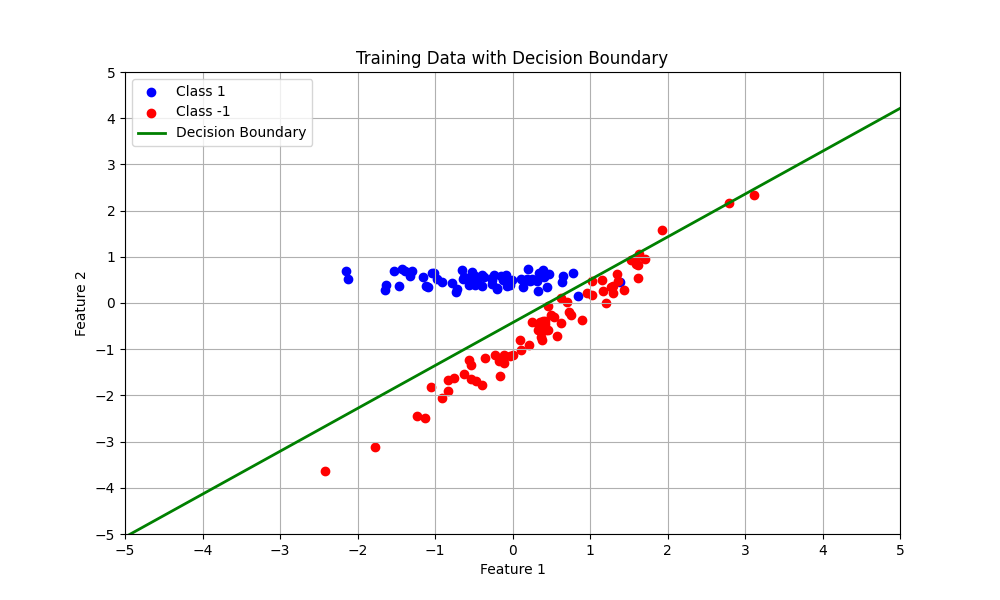
\includegraphics[width=\textwidth]{output/dataset1/train_decision_boundary.png}
        \caption{Training Data}
    \end{subfigure}
    \hfill
    \begin{subfigure}[b]{0.48\textwidth}
        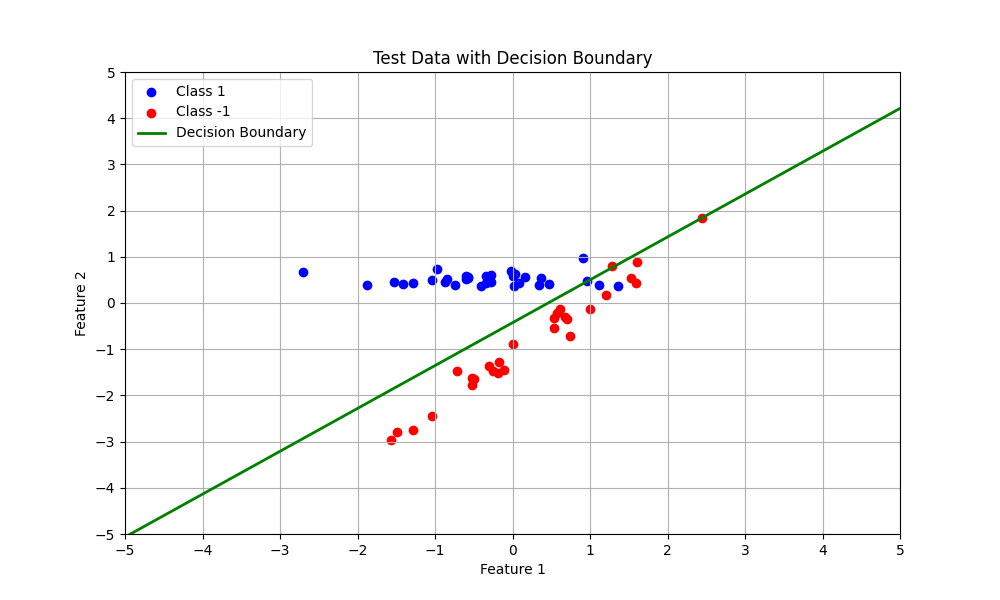
\includegraphics[width=\textwidth]{output/dataset1/test_decision_boundary.png}
        \caption{Test Data}
    \end{subfigure}
    \caption{Dataset 1: Decision Boundary}
\end{figure}

\section{Dataset 2}

\subsection{Results}
\begin{itemize}
    \item \textbf{Training Accuracy (Last Epoch):} 49.71\%
    \item \textbf{Test Accuracy:} 68.00\%
\end{itemize}

\subsection{Analysis}
The performance on Dataset 2 was poor, with accuracy hovering around random guessing (50-60\%). This is expected due to the geometric distribution of the data. 

The dataset consists of two classes arranged in a concentric manner: one class forms a smaller inner circle, while the other forms a surrounding ring (disk). This distribution is inherently \textbf{non-linearly separable}. Since the Perceptron is a linear classifier, it can only draw a straight line to separate the classes. It is impossible to separate a circle from a ring with a single straight line, resulting in the high classification error and the "cut-through" decision boundary seen in the plots.

\begin{figure}[H]
    \centering
    
\includegraphics[width=0.7\textwidth]{output/dataset2/training_error.png}
    \caption{Dataset 2: Training Error Evolution}
\end{figure}

\begin{figure}[H]
    \centering
    \begin{subfigure}[b]{0.48\textwidth}
        
\includegraphics[width=\textwidth]{output/dataset2/train_decision_boundary.png}
        \caption{Training Data}
    \end{subfigure}
    \hfill
    \begin{subfigure}[b]{0.48\textwidth}
        
\includegraphics[width=\textwidth]{output/dataset2/test_decision_boundary.png}
        \caption{Test Data}
    \end{subfigure}
    \caption{Dataset 2: Decision Boundary (Linear Attempt on Non-Linear Data)}
\end{figure}

\section{Dataset 3}

This dataset has 10 attributes, so decision boundaries cannot be visualized in 2D. We performed a grid search over Learning Rate (LR) and Epochs, repeating each configuration 20 times to calculate mean accuracy and standard deviation.

\subsection{Results Summary}

\begin{table}[H]
    \centering
    \begin{tabular}{|c|c|c|c|}
        \hline
        \textbf{Learning Rate} & \textbf{Epochs} & \textbf{Mean Test Accuracy} & \textbf{Std Deviation} \\
        \hline
        0.01 & 100 & 83.97\% & 2.40\% \\
        0.01 & 200 & 83.17\% & 1.77\% \\
        0.01 & 400 & 84.29\% & 2.18\% \\
        \hline
        0.1 & 100 & 82.70\% & 2.70\% \\
        0.1 & 200 & 84.29\% & 3.51\% \\
        0.1 & 400 & 83.81\% & 2.91\% \\
        \hline
        0.5 & 100 & 83.17\% & 3.11\% \\
        0.5 & 200 & 83.97\% & 2.50\% \\
        0.5 & 400 & 83.81\% & 2.33\% \\
        \hline
    \end{tabular}
    \caption{Performance on Dataset 3 with varying hyperparameters (20 runs)}
\end{table}

\subsection{Analysis}
\begin{itemize}
    \item The highest mean test accuracy (84.29\%) was achieved with $\eta=0.1$ (200 epochs) and $\eta=0.01$ (400 epochs).
    \item \textbf{High Variance:} All configurations show a standard deviation between 1.77\% and 3.51\%, indicating that the final accuracy depends somewhat on the random initialization of weights.
    \item \textbf{Stability:} Increasing epochs to 400 yielded consistent results across different learning rates, suggesting convergence.
\end{itemize}

\subsection{Training Error Plots}

\begin{figure}[H]
    \centering
    \begin{subfigure}[b]{0.32\textwidth}
        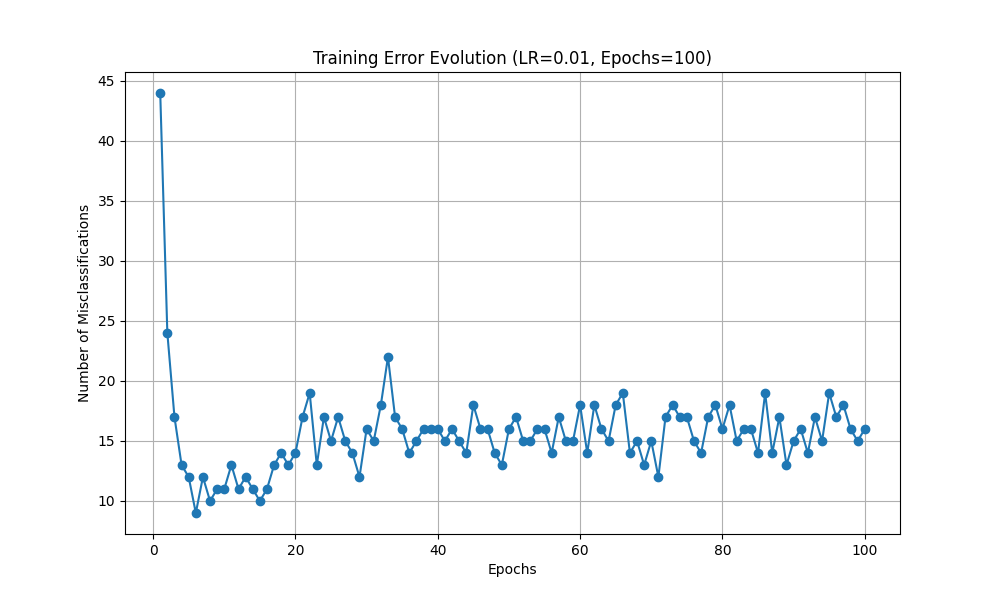
\includegraphics[width=\textwidth]{output/dataset3/training_error_lr_0.01_epochs_100.png}
        \caption{LR=0.01, Epochs=100}
    \end{subfigure}
    \hfill
    \begin{subfigure}[b]{0.32\textwidth}
        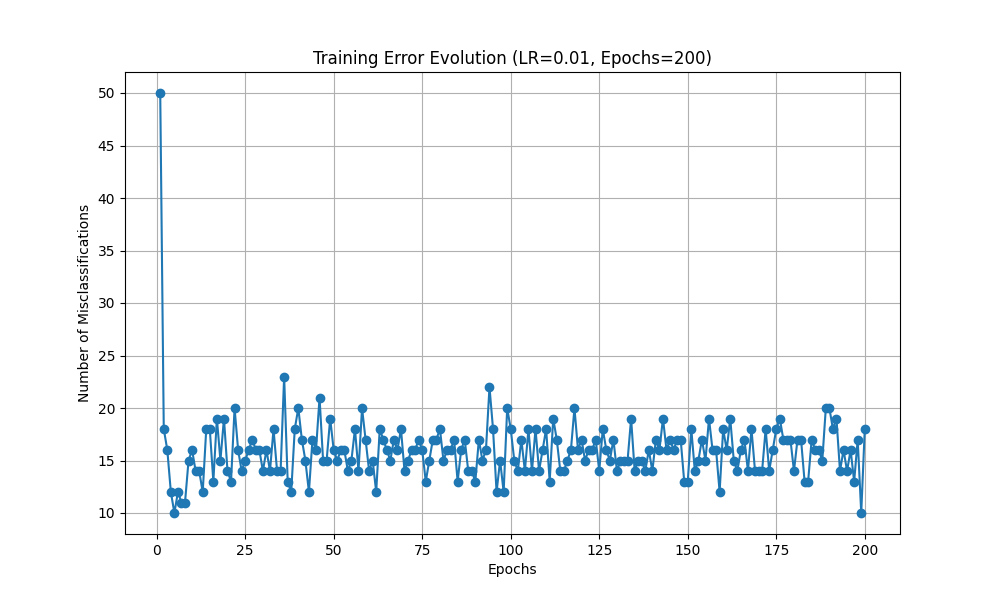
\includegraphics[width=\textwidth]{output/dataset3/training_error_lr_0.01_epochs_200.png}
        \caption{LR=0.01, Epochs=200}
    \end{subfigure}
    \hfill
    \begin{subfigure}[b]{0.32\textwidth}
        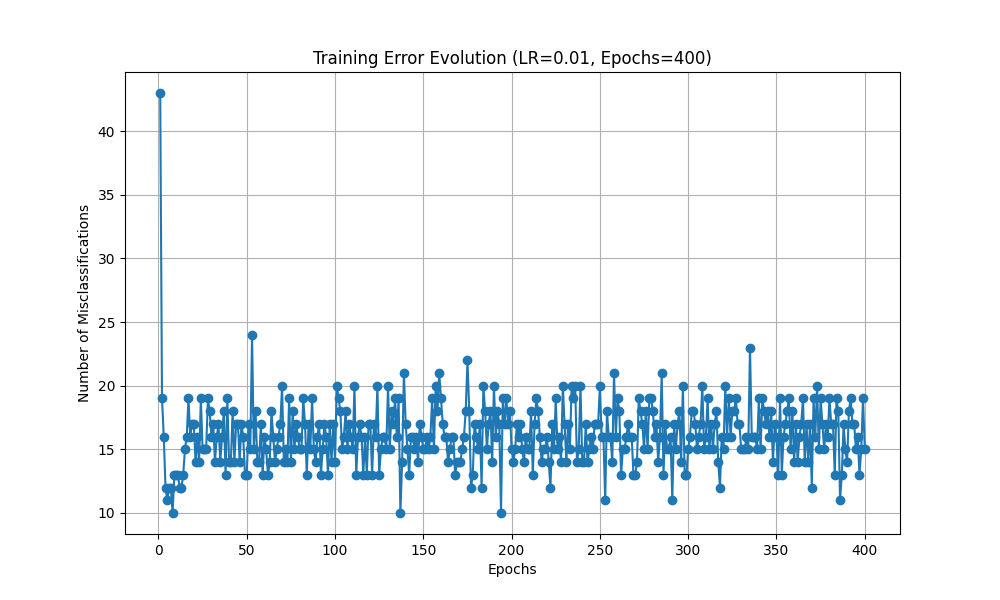
\includegraphics[width=\textwidth]{output/dataset3/training_error_lr_0.01_epochs_400.png}
        \caption{LR=0.01, Epochs=400}
    \end{subfigure}
    
    \begin{subfigure}[b]{0.32\textwidth}
        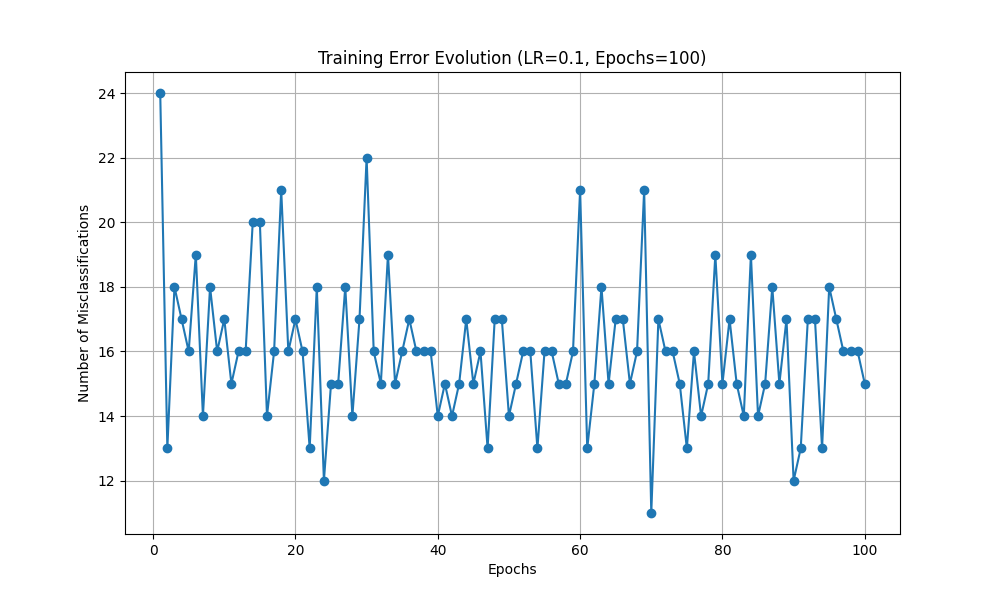
\includegraphics[width=\textwidth]{output/dataset3/training_error_lr_0.1_epochs_100.png}
        \caption{LR=0.1, Epochs=100}
    \end{subfigure}
    \hfill
    \begin{subfigure}[b]{0.32\textwidth}
        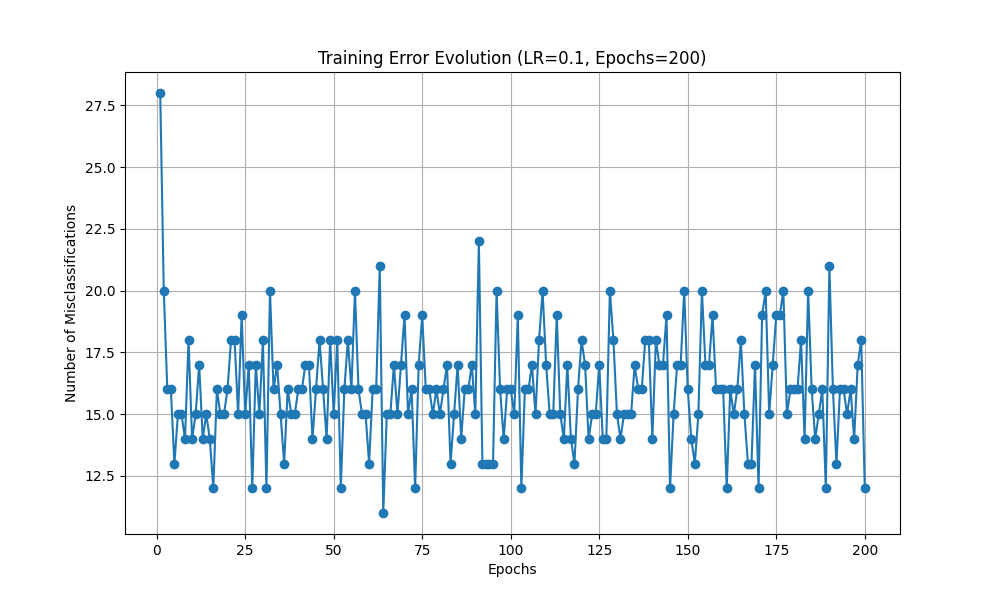
\includegraphics[width=\textwidth]{output/dataset3/training_error_lr_0.1_epochs_200.png}
        \caption{LR=0.1, Epochs=200}
    \end{subfigure}
    \hfill
    \begin{subfigure}[b]{0.32\textwidth}
        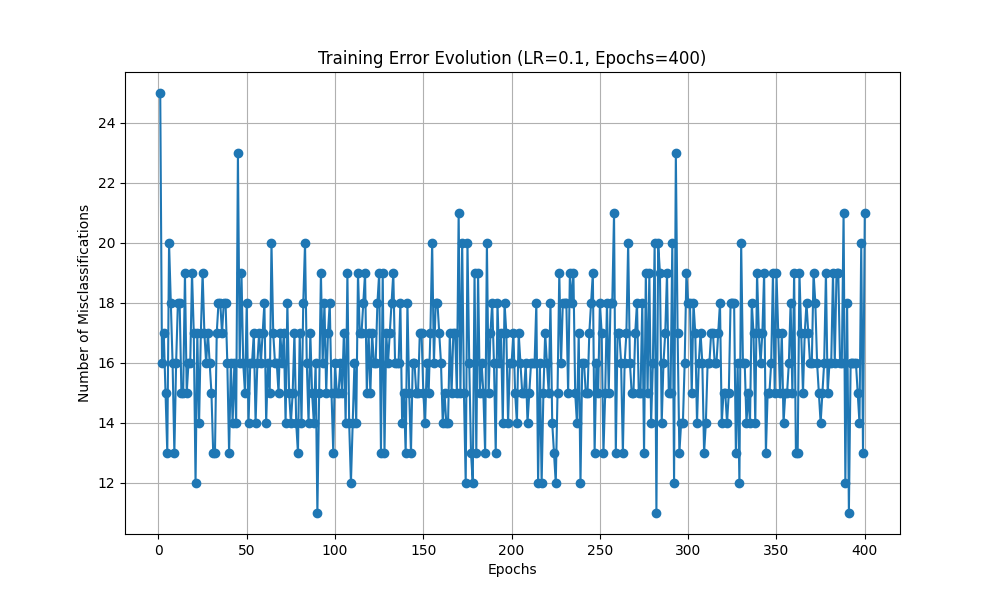
\includegraphics[width=\textwidth]{output/dataset3/training_error_lr_0.1_epochs_400.png}
        \caption{LR=0.1, Epochs=400}
    \end{subfigure}

    \begin{subfigure}[b]{0.32\textwidth}
        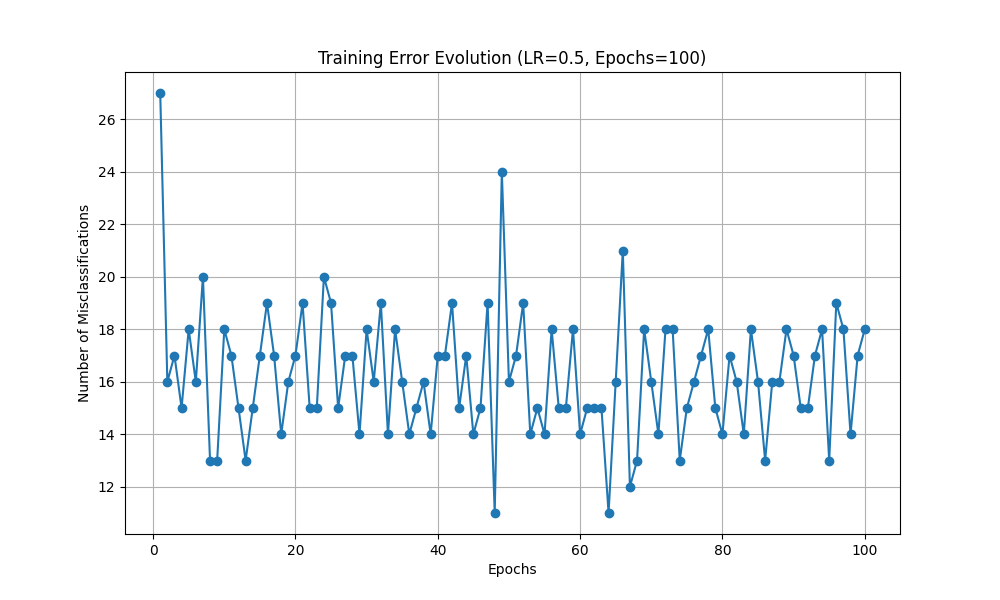
\includegraphics[width=\textwidth]{output/dataset3/training_error_lr_0.5_epochs_100.png}
        \caption{LR=0.5, Epochs=100}
    \end{subfigure}
    \hfill
    \begin{subfigure}[b]{0.32\textwidth}
        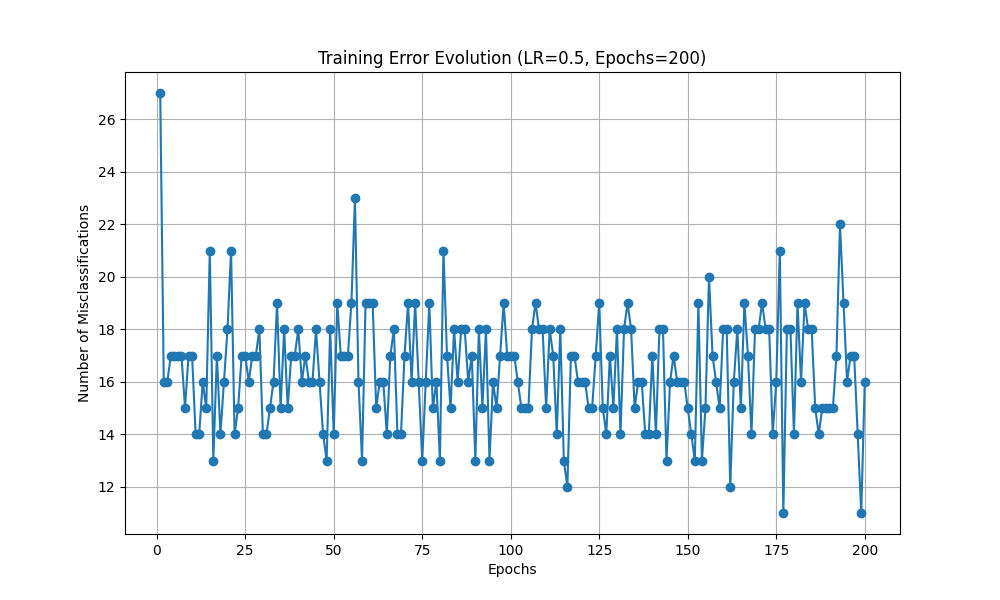
\includegraphics[width=\textwidth]{output/dataset3/training_error_lr_0.5_epochs_200.png}
        \caption{LR=0.5, Epochs=200}
    \end{subfigure}
    \hfill
    \begin{subfigure}[b]{0.32\textwidth}
        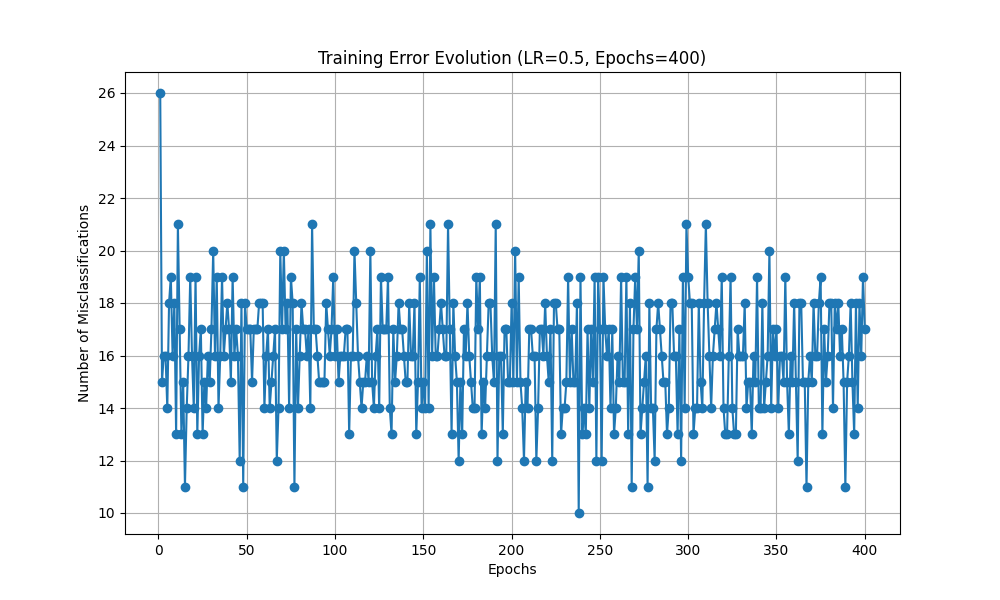
\includegraphics[width=\textwidth]{output/dataset3/training_error_lr_0.5_epochs_400.png}
        \caption{LR=0.5, Epochs=400}
    \end{subfigure}
    \caption{Training Error Evolution for different hyperparameters (Dataset 3)}
\end{figure}

\end{document}
